\begin{example}[Diffusion 2D]
\label{ex:laplace}
Inspired by \cite[cv. 8.4 (3), p. 150]{Holubova2011}, in $\Omega = \langle 0, 1 
\rangle^2$ 
we will solve Laplace equation \eqref{eq:ex_laplace}.
%\begin{equation}
%\pdiff{^2 u}{x^2} + \pdiff{^2 u}{y^2} = 0
%\end{equation}
%i.e
%\begin{equation}
%\Delta u = 0.
%\end{equation}
We setup boundary condition in such way that the exact solution 
$u_{exact}$ is polynomial
\begin{equation}
u_{exact} = \frac{1}{2}x^2 - \frac{1}{2}y^2 - ax + by + c.
\end{equation}
We set boundary conditions to match analytical solution as follows
\begin{equation}
	\begin{aligned}
		&u_x(0, y) = -a, & u_x(a, y) = 0\\
		&u_y(x, 0) = b, & u_y(x, b) = 0.
	\end{aligned}
\end{equation}
In our setting we chose $a=1$, $b=1$, $c=0$. Different values of 
coefficient $C_w$ in penalty term yield different convergence behavior as demonstrated in 
Figures \ref{fig:conv_laplace} and \ref{fig:orders_lapalce}.  \Cref{fig:orders_lapalce} 
may suggest that high order method do not meet expected convergence rate, they however 
still attain lowest error as illustrated in \Cref{fig:conv_laplace}. This is due to 
the polynomial solution which can be approximated very accurately even on coarse mesh and 
refining does not provide much benefit especially for high order approximations.
\end{example}

\begin{figure}[h!]
	\centering
	\begin{tabular}{p{0.5\textwidth} p{0.5\textwidth}}
		\vspace{0pt} 
        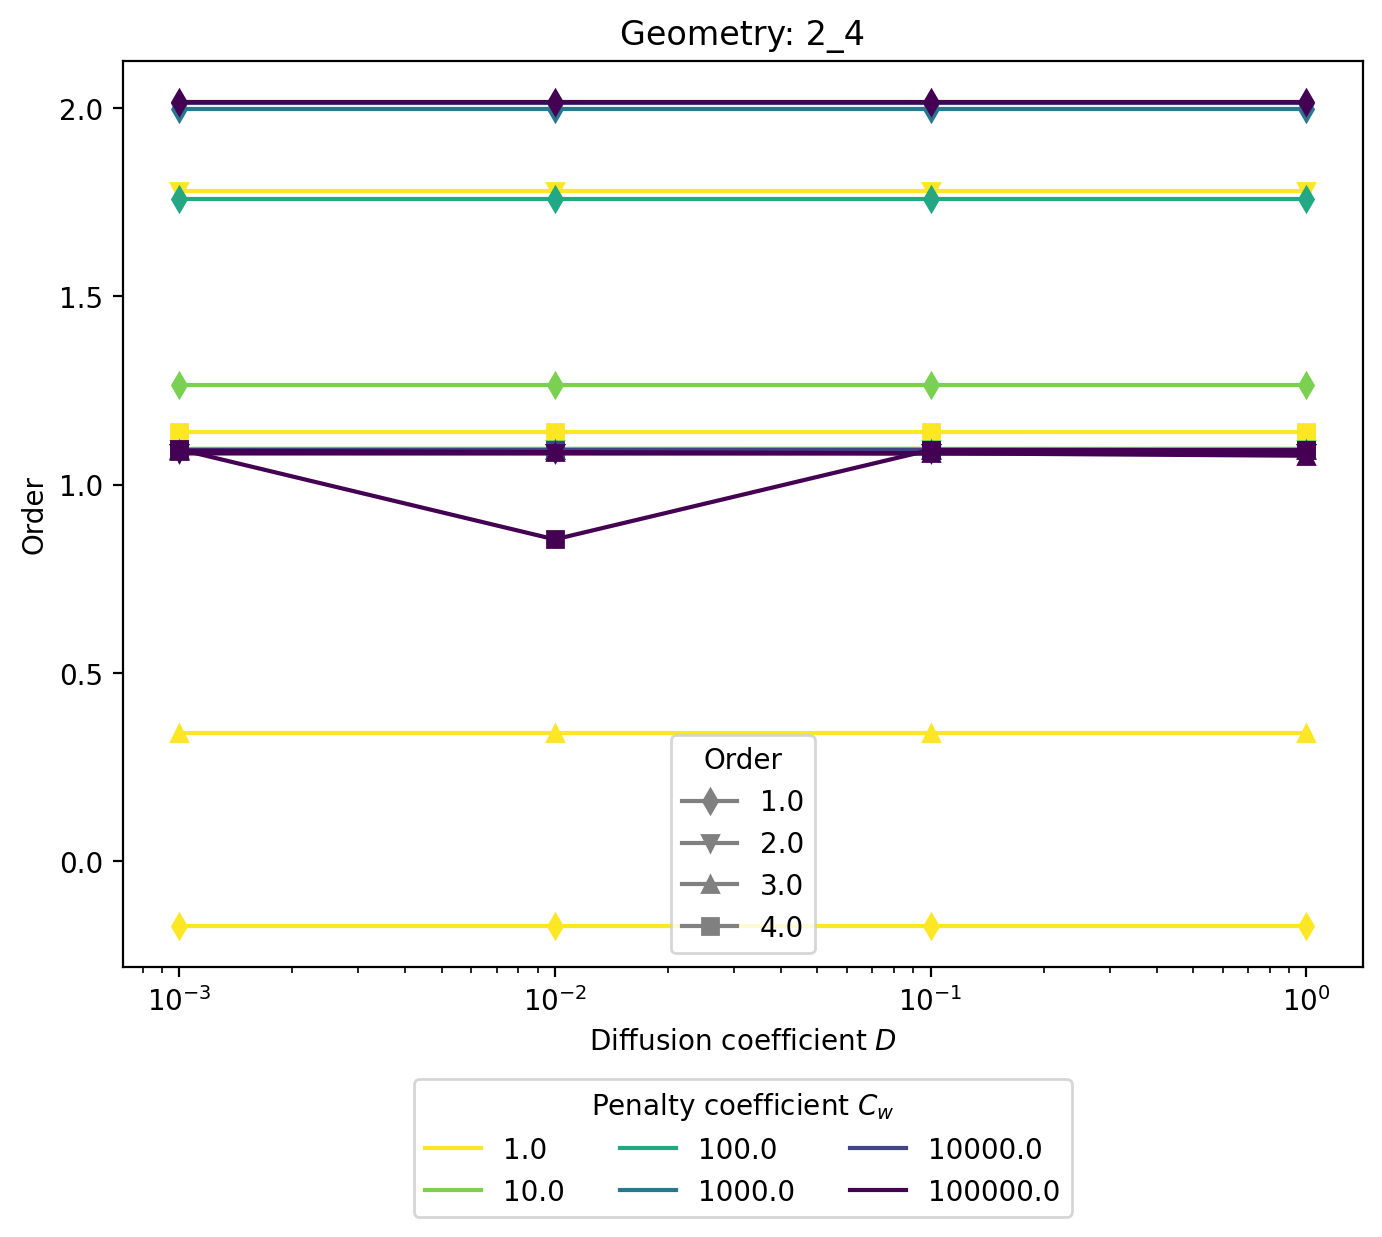
\includegraphics[width=0.49\textwidth]{../figs/parametric/diffusion_2D/ord_laplace_2_4}
		&
		\vspace{0pt} 
        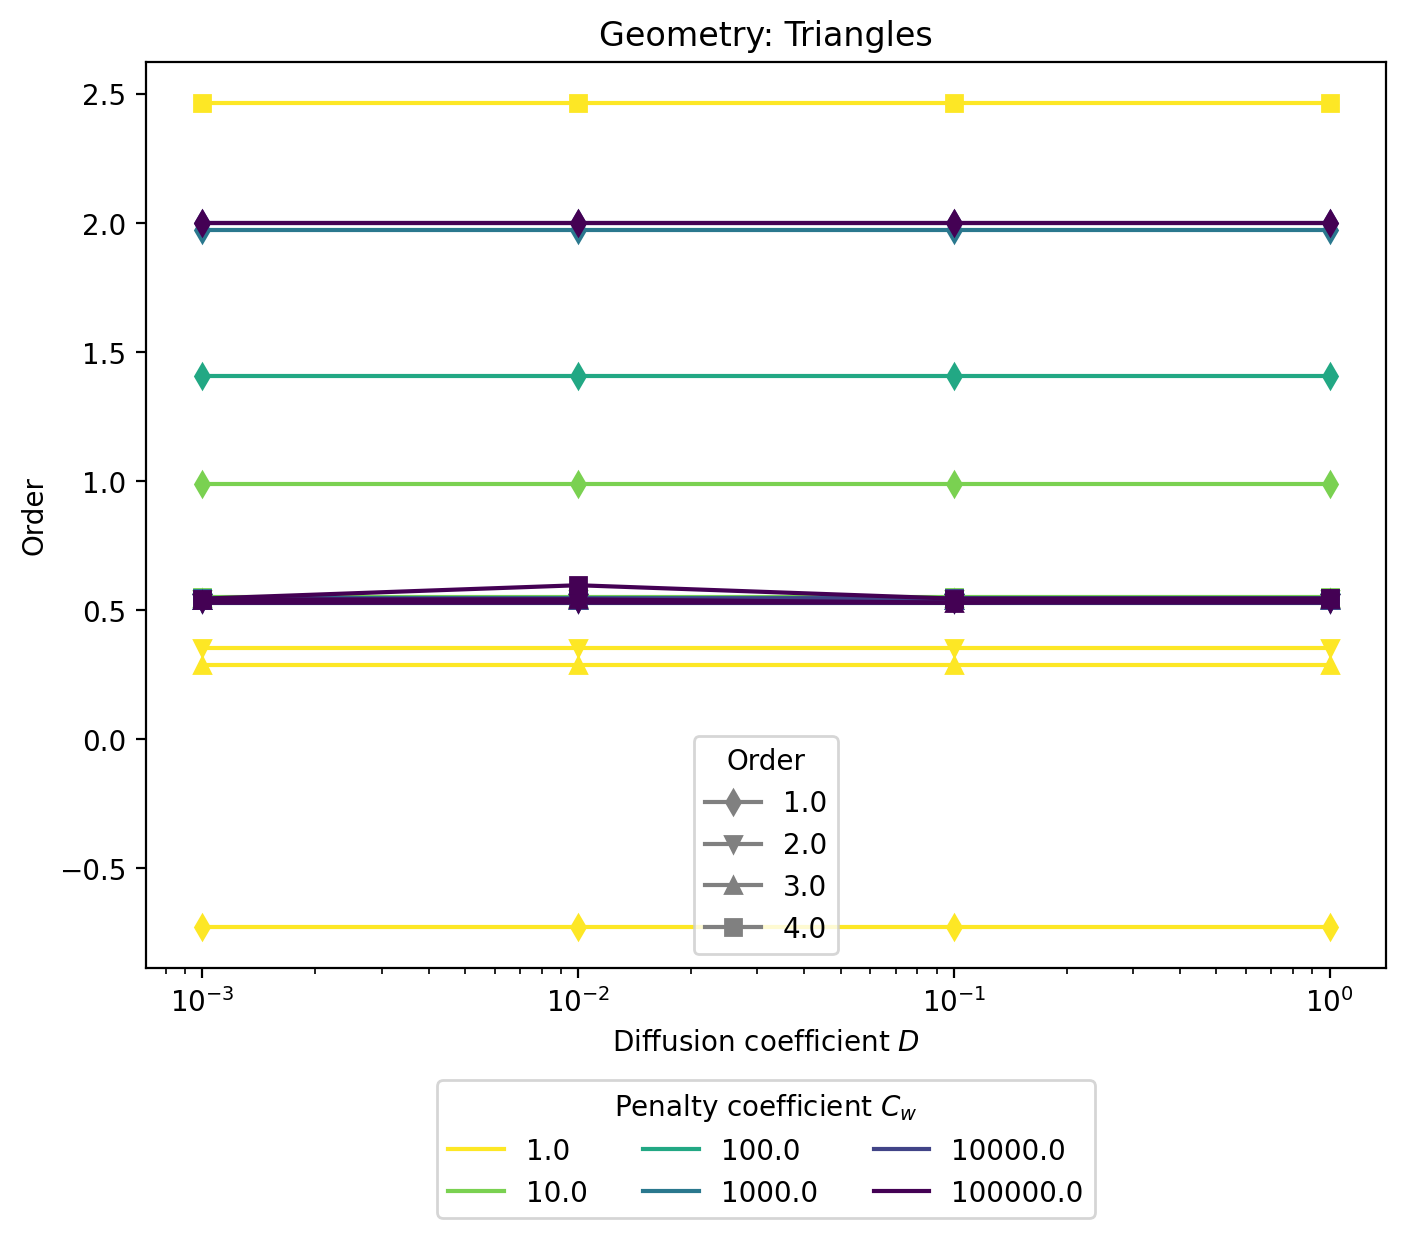
\includegraphics[width=0.49\textwidth]{../figs/parametric/diffusion_2D/ord_laplace_2_3}
	\end{tabular}
	\caption{\Cref{ex:laplace}. Average convergence rates for different choices of $C_w$ 
	for quadrilaterals (left) and triangles (right).}
	\label{fig:orders_lapalce}
\end{figure}

%\begin{figure}[h!]
%	\centering
%	\begin{subfigure}{.5\textwidth}	
%		\centering		
%        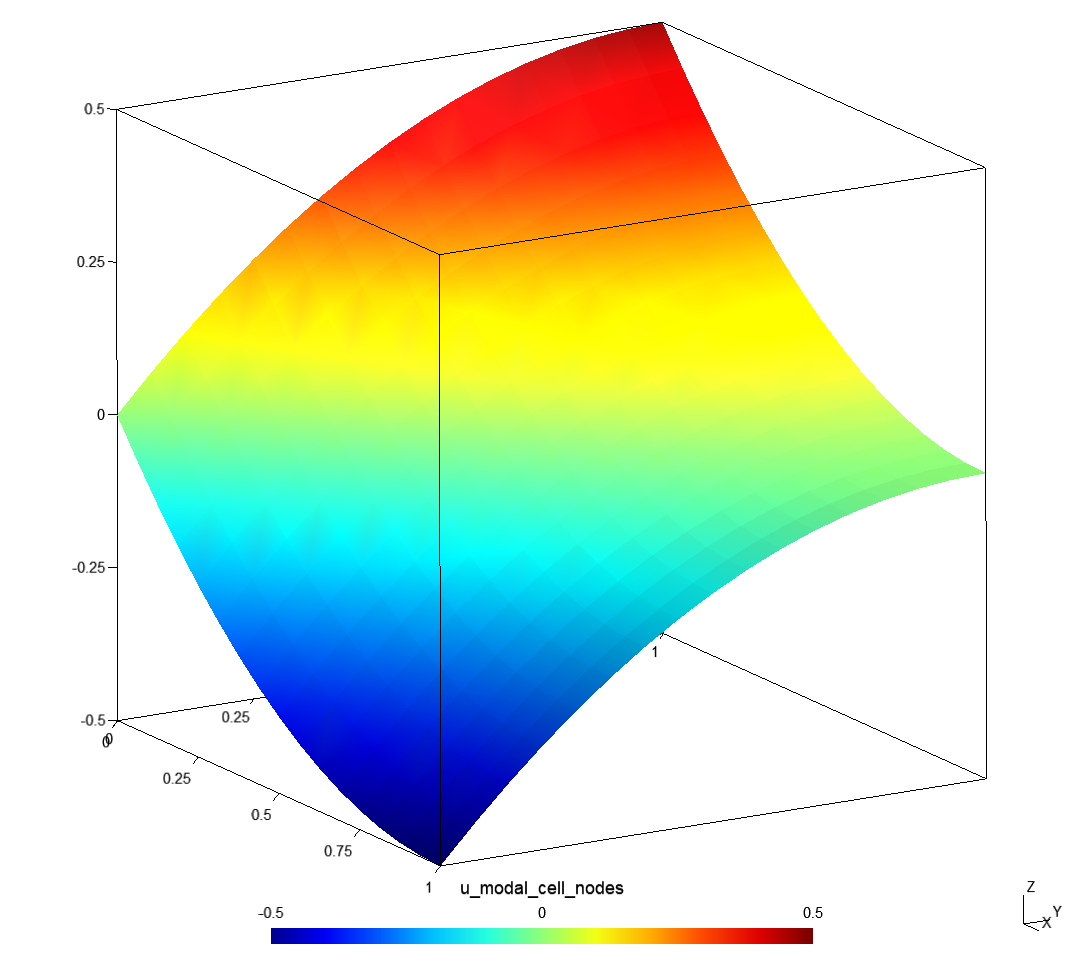
\includegraphics[width=\linewidth]{../figs/sols/laplace-52000-sol-h256o03.png}
%		\caption{??}
%	\end{subfigure}%
%%	\begin{subfigure}{.5\textwidth}
%%		\centering	
%%\includegraphics[width=\linewidth]{../figs/sols/}
%%		\caption{$C_w = 15$}
%%	\end{subfigure}
%	\caption{Solutions of \Cref{ex:laplace}  }
%\end{figure}

\begin{figure}[p!]
	\centering
	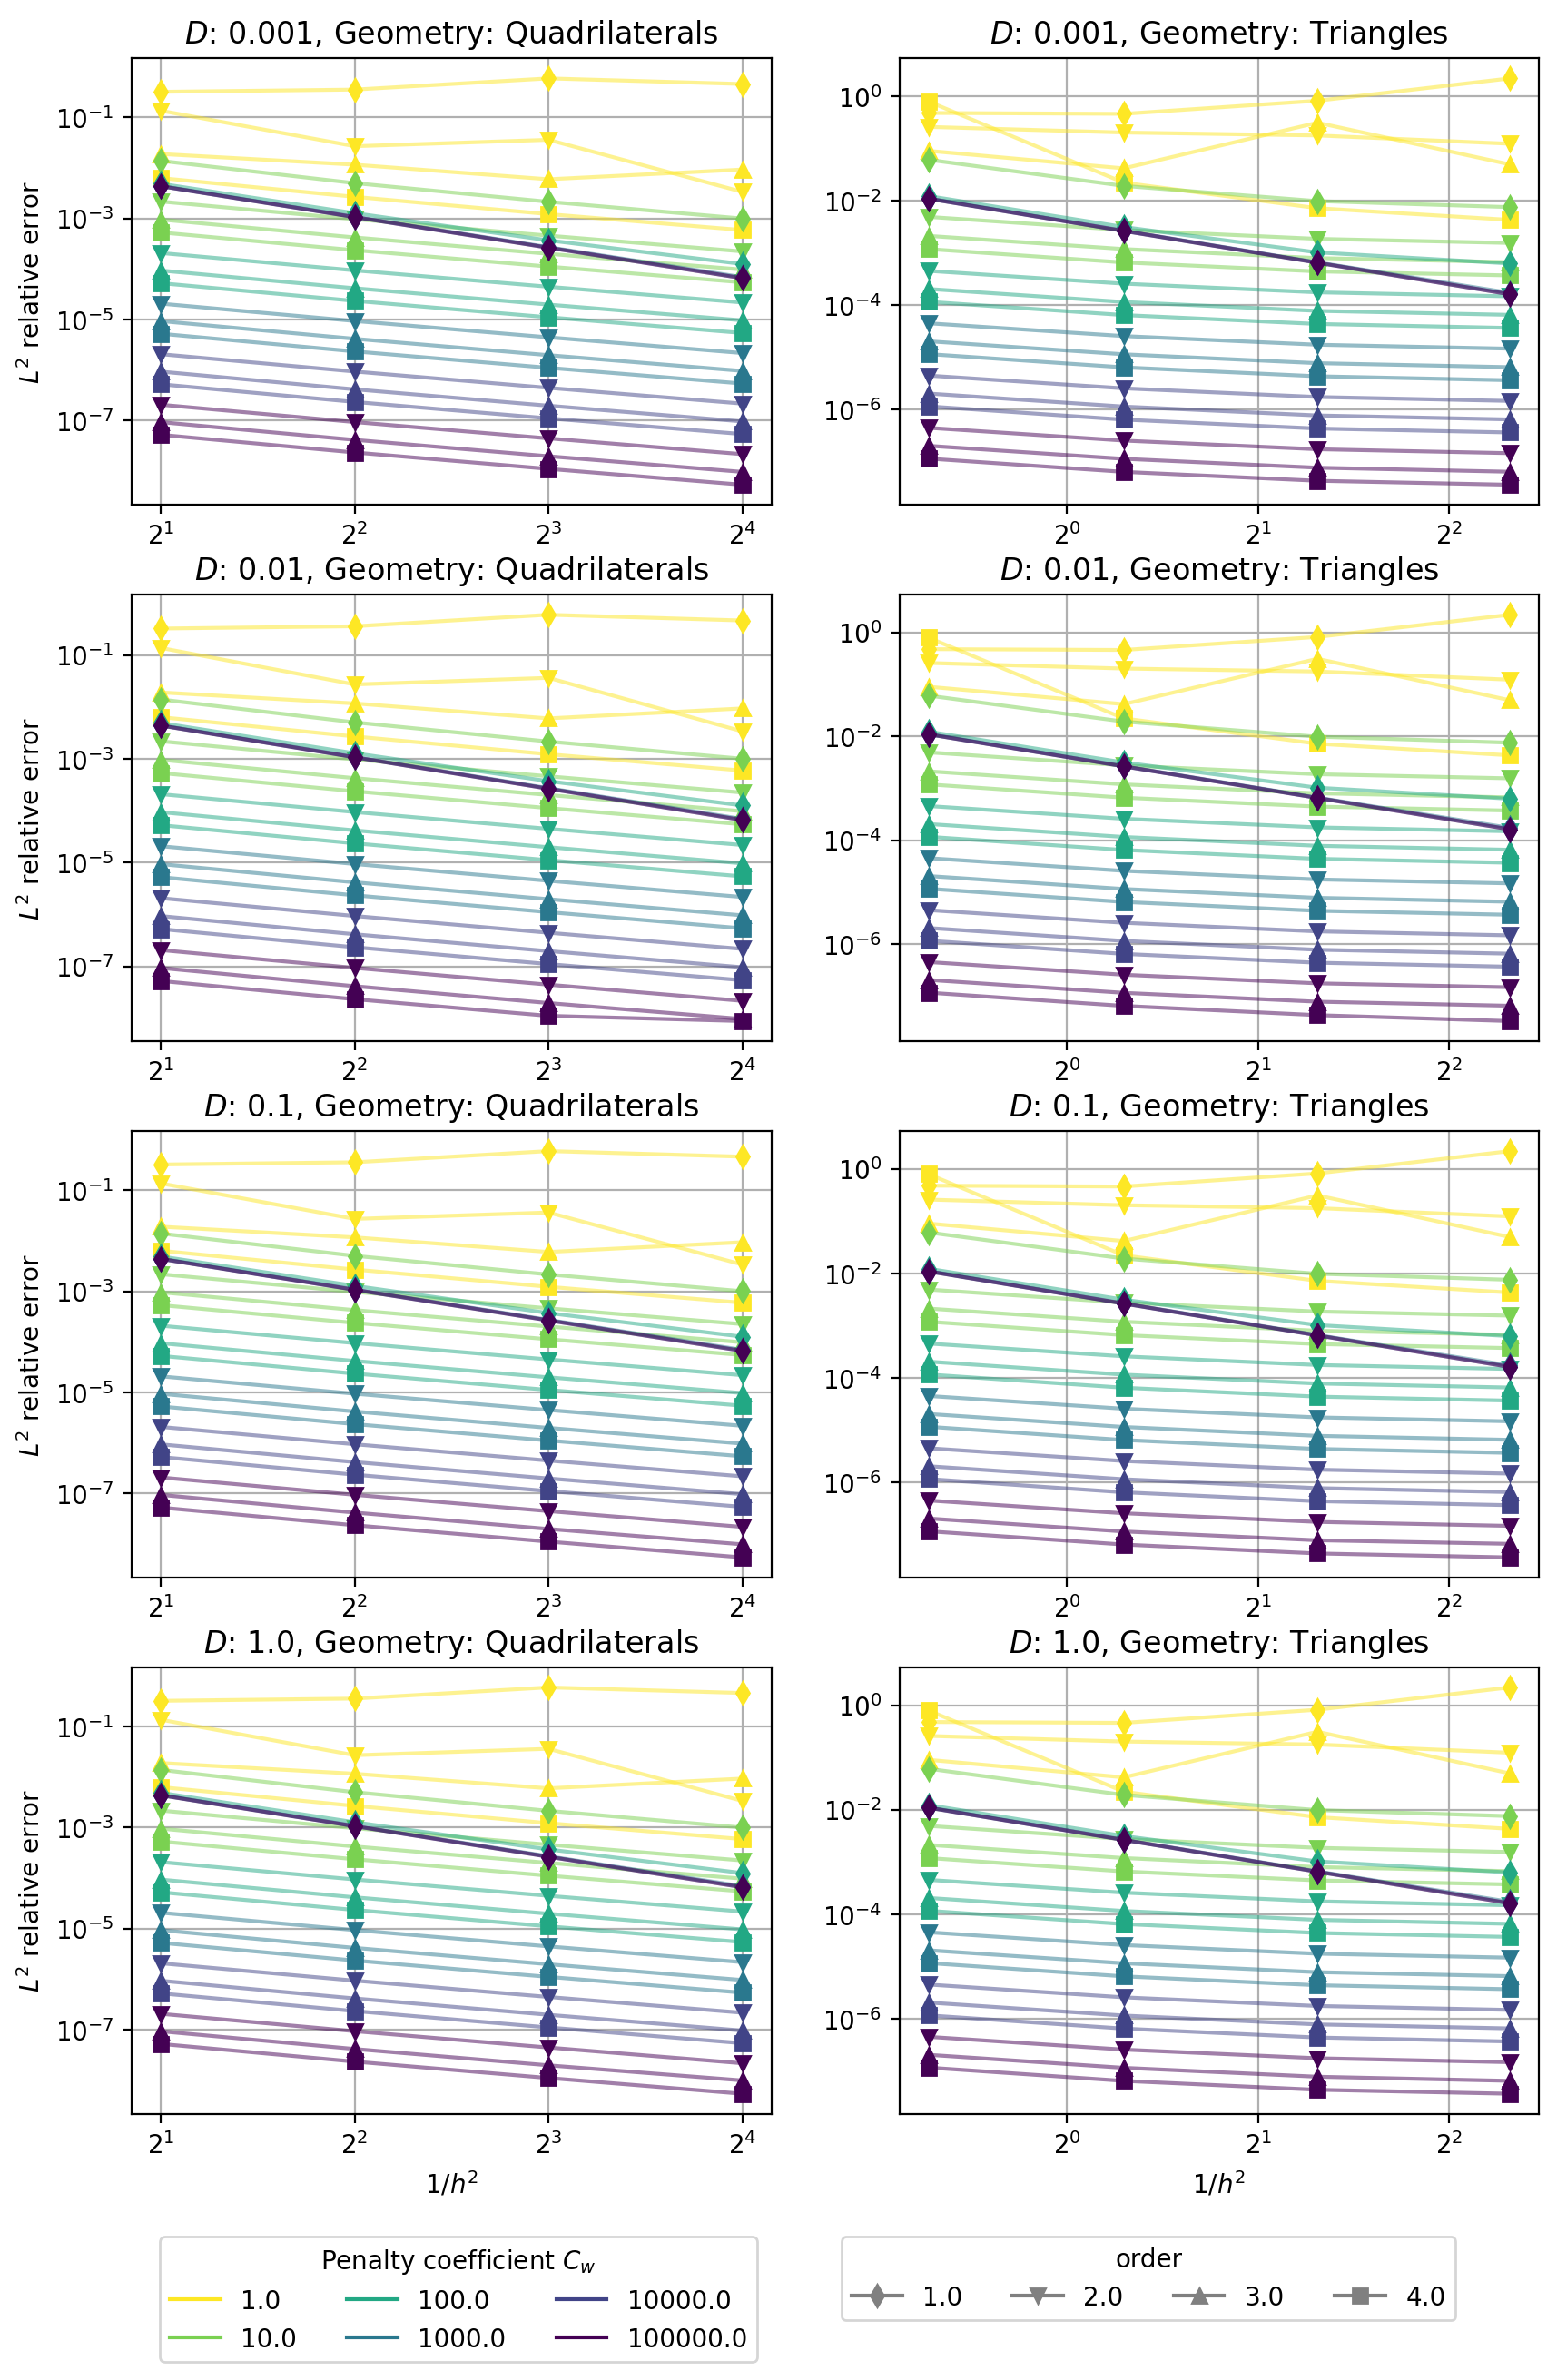
\includegraphics[height=\textheight]{../figs/parametric/diffusion_2D/laplace.png}
	\caption{\Cref{ex:laplace}. Relative errors for different choice of $C_w$  for 
		quadrilaterals (left) and triangles (right).}
	\label{fig:conv_laplace}
\end{figure}